%Correct the file name.
%X: book number
%Y: part number
%ZZZ: page number in three digits. So page 3 would be 003.

\documentclass[11pt]{amsbook}

\usepackage{../HBSuerDemir}	% ------------------------


\begin{document}


% ++++++++++++++++++++++++++++++++++++++
\hPage{vol-1/91}
% ++++++++++++++++++++++++++++++++++++++




	\begin{center}
		\section{Subgroups}
	\end{center}

	\begin{par}
		\noindent A group is a set with a binary operation on it which has some nice properties. Being a set, a group has subsets. Naturally, we are more 
		interested in those subsets which reflect the algebraic structure of the group than in the other subsets.They help us understand the structure
		of the group. Foremost among them are the sets which are groups themselves. We give them a name.
	\end{par}

		\hspace{1pt}

	\begin{defn}
		Let $G$ be a group. A nonempty subset $H$ of  $G$ is a subgroup of  $G$ if  $H$ itself is a group under the operation on $G$.
	\end{defn}

	\hspace{1pt}
	
	\begin{par}
		\noindent We write $H\leq G$ to express that $H$ is a subgroup of $G$.Clearly, $G$ is a subgroup of $G$, so $G \leq G$. If $H$ is a subgroup of $G$ and a proper 		    		
		subset of $G$, i.e., if $H \leq G$ and $H \subset G$, we call $H$ a proper subgroup of $G$.  In this case, we write $H < G$.The notations $H \nleq G$ and 
		$H \nless G$ mean that $H$ is not a subgroup respectively not a proper subgroup of $G$.
	\end{par}
	
	\hspace{1pt}
	
	\begin{par}
		\noindent Given a group $G$ and a nonempty subset $H$ of $G$, we must check the group axioms for $H$ in order to determine whether $H$ is a subgroup of $G$. We now discuss each one of these axioms. It turns out that we can do without some of them.
	\end{par}
	
	\hspace{1pt}
	
	\begin{par}
		\noindent First of all, there must be a binary operation on $H$. The operation on $H$ is the operation on $G$. More precisely, the operation on $H$ is the restriction of the operation on $G$ to $H$. 
		Hence, for $a,b \in H$, the element $ab$ is computed asthe product of $a$ and $b$ in $G$. 
		In order to have a binary operation on $H$, given by $ (a,b) \Rightarrow ab $ as in $G$, it is necessary and sufficient that $ab \in H$ for all $a,b \in H $. Hence
		$H$ must be closed under the multiplicaiton on $G$. Then and only then is there a binary operation on $H$ that is the restriction of the multiplication on $G$.
	\end{par}
\end{document}  

%==== templates ====

%==== environments ====

%\begin{figure}[htb]
%	\centering
%	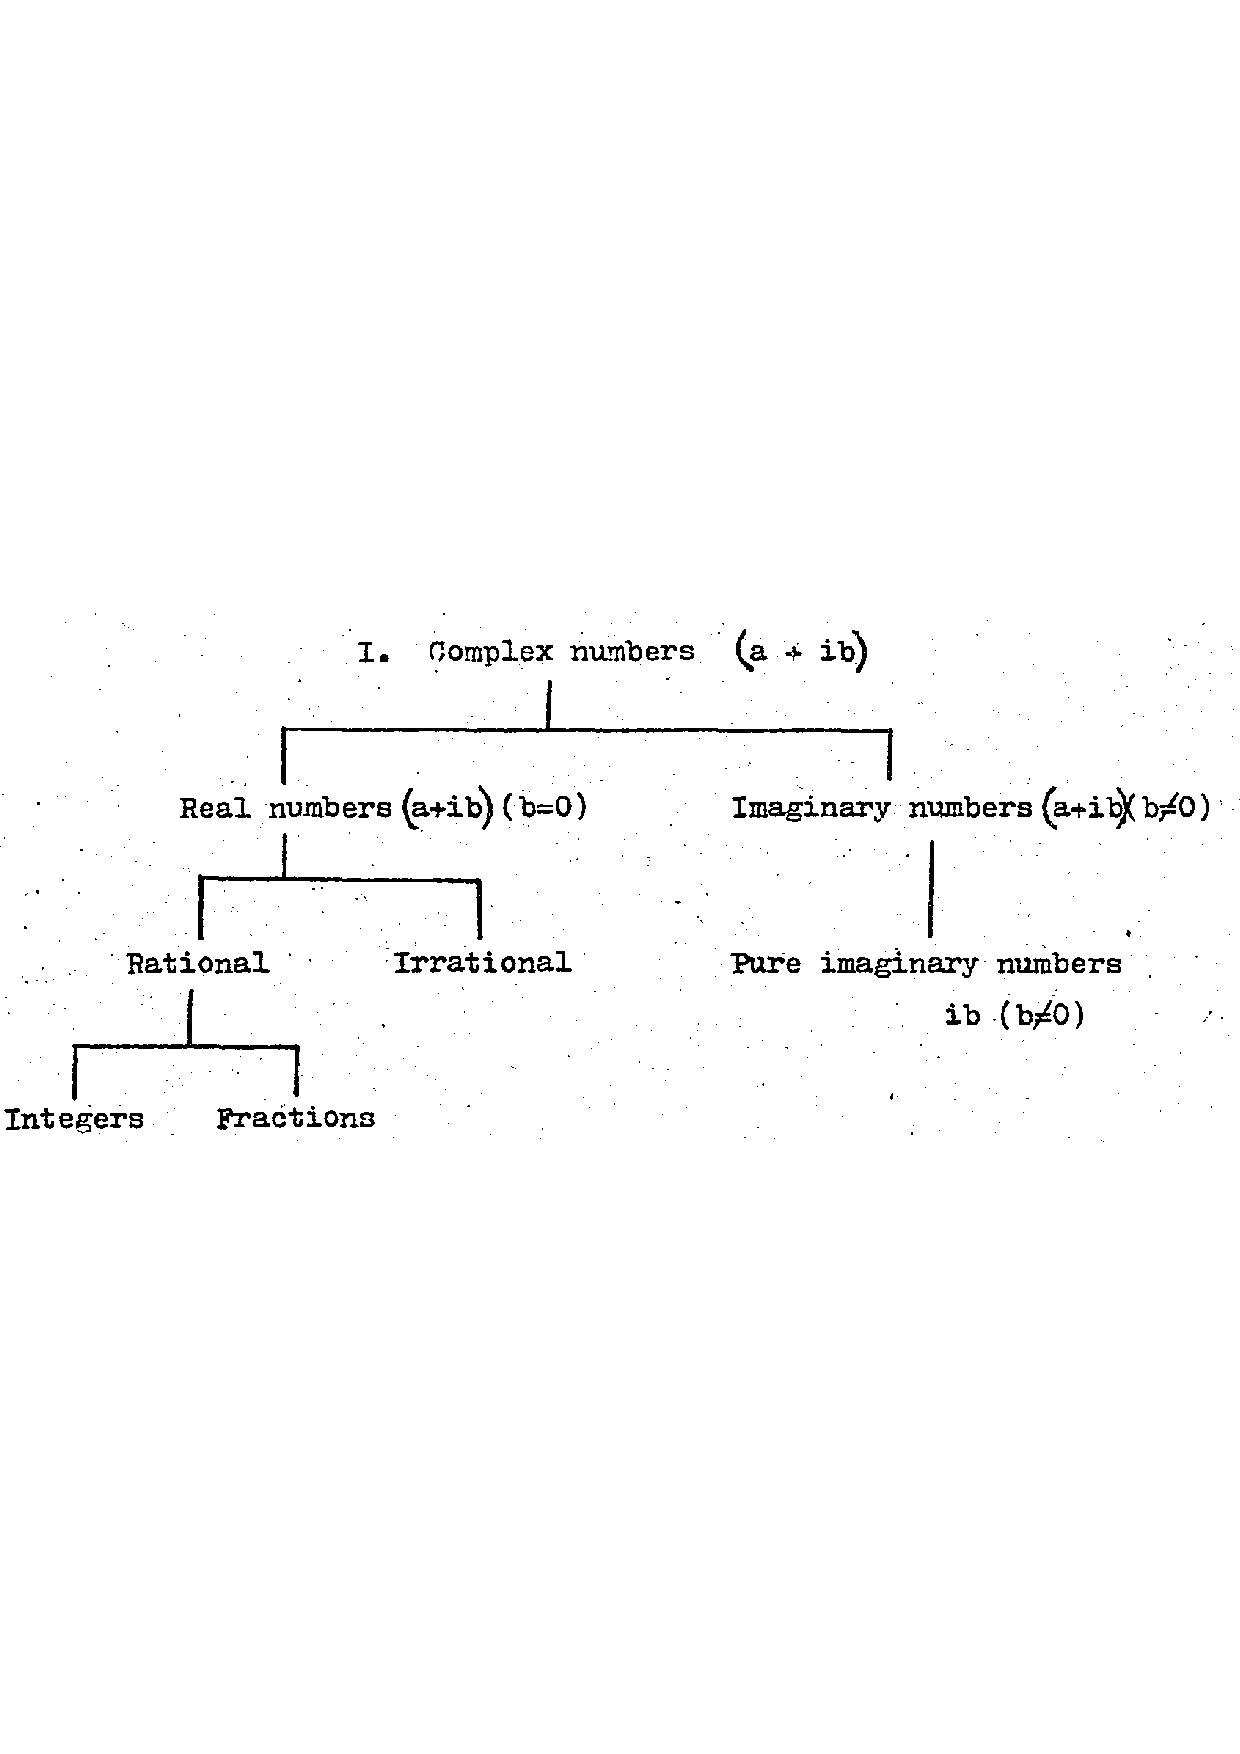
\includegraphics[width=0.9\textwidth]{images/SD-1-1p15A}
%	\caption{Classification of complex numbers}
%	\label{fig:classificationOfComplexNumbersA}
%\end{figure}

%\begin{center}
%\begin{tabular}{cc}
%\end{tabular}
%\end{center}

%\begin{exmp}
%\begin{hSolution}
%\end{hSolution}
%\end{exmp}

%\begin{hEnumerateAlpha}
%\end{hEnumerateAlpha}

%\begin{hEnumerateRoman}
%\end{hEnumerateRoman}

%$
%\begin{bmatrix}
%\end{bmatrix}
%$

%\frac{aaaa}{bbb}
%\frac{a_{n}}{b_{n}}
%\left( aaaa \right)
%\Longrightarrow

%\begin{multicols}{2}
%	bb
%\columnbreak
%	aa
%\end{multicols}
